\chapter{Evaluation} \label{sec:evaluate_scheduling}

\section{Parameter Description}

In order to evaluate the carbon savings made possible by the previously established dynamic power model, the following approach is proposed:
As the already existing job traces hold no information regarding the power or their phases, some test cases will be presented and used for the models.
In a rather explorative process, we use the following parameters and run the simulation on all possible permutations of them. 
This is done using the \verb|generate_evaluation_jobs.sh| script, the used parameters are listed in the following table:

\begin{table}[h!]
    \centering
    \begin{tabular}{|p{0.3\linewidth}|p{0.6\linewidth}|}
    \hline
        Parameter & Values \\ \hline
        Scheduling Strategy & suspend \& resume, non-interrupted \\ \hline
        Phases & alternating high- and low-powered phases, each either 30 or 60 minutes long \\ \hline
        Startup length & no startup, 5 minutes, 10 minutes, 30 minutes \\ \hline
        Startup power level & 100 W, 200 W \\ \hline
        Waiting time & 4 hours, 12 hours, 1 day, 2 days \\ \hline
        Job length & 1, 2, and 3 hours \\ \hline
        Carbon trace & Week from July 1. 2024 (see Figure \ref{fig:energy_mix}) \\ \hline
    \end{tabular}
    \caption{Overview of the parameters used for the evaluation}
    \label{tab:evaluation_parameters}
    \end{table}

Another dimension will be comparing these scenarios against having no information on phases, instead only having an averaged constant wattage of the otherwise existing phases.
The latter represents the previous \verb|GAIA| implementation, where jobs had a constant amount of power at all points in time.
Finding the LP solution will time-limited to 20 minutes and all jobs will be simulated to be submitted at the very first time in the trace.

\todo[inline]{This needs some better explanation, the phases don't really make too much sense, perhaps just go with the generic ML-job setup I introduced earlier}

\section{Running the Evaluation on a Cluster}

As previously discussed in Section \ref{sec:checkpoint_resume_lp}, calculating suspend \& resume scheduling tends to have high runtime and memory requirements. 
For that reason, the simulation was executed on the \emph{SCORE Lab}, short for \emph{scientific compute resources}, of HPI.

After requesting and gaining access, \verb|rsync| was used to transfer the simulation to the cluster. 
Slurm could then be used to schedule all experiments individually (that were generated using the mentioned \verb|generate_all_jobs.sh| script), which would parallelize the evaluation, leading to faster results.

One problem arose in the licensing of the used \emph{Gurobi} solver. 
Under our academic license, only 2 \emph{sessions} are allowed simultaneously.
A session is defined via the hostname of the executing machine, which is communicated to the solver's licensing servers live.
As such, scheduling each experiment by itself lead to many sessions being started, as Slurm distributes the jobs on the available nodes.
While there is some leeway in the amount of sessions, experiments crashed beyond the 5th instance as the solver did not start.

We work under this restriction by distributing the experiments across two workers (via a script called \verb|evalute_dynamic_power.sh|); as each experiment has an index, one worker executes the even numbered jobs and the other executes the odd ones. 
Using the even-odd strategy results in both workers having about the same amount of work.

The workers in this case are python docker containers that were created with the help SCORE Lab's online knowledge base.\webcite{web_knowledgebase}
The command for launching one example worker, in this case the one for even jobs, is given in Listing \ref{list:evaluation_slurm}.

\begin{minipage}{\linewidth}
\begin{lstlisting}[language=bash, frame=single, numbers=left, caption={Executing the Evaluation inside the SCORE Lab's Slurm environment}, label={list:evaluation_slurm}, basicstyle=\ttfamily]
    sbatch -A polze -p magic \
        --container-image=python \
        --container-name=test \
        --container-writable \
        --mem=128G \
        --cpus-per-task=128 \
        --time=24:0:0 \
        --output=slurmlogs/output_%j.txt \
        --error=slurmlogs/error_%j.txt \
        --constraint=ARCH:X86 \
        --container-mounts=/hpi/fs00/home/vincent.opitz:/home/vincent.opitz \
        --container-workdir=/home/vincent.opitz/master-thesis/GAIA \
        run_all_even_jobs.sh
        \end{lstlisting}    
\end{minipage}

Now the simulation can be run with 128 GB RAM as specified in line 5. 
The \verb|-p magic| parameter results in us using a compute node. 
Line 3, \verb|--container-writable|, means that the container will be reused if called again under the same name, this lets us conduct set up  (\verb|pip install|).
Restricting the nodes to be \verb|X86| nodes via line 10 is necessary as there are other architectures available in the cluster. 
Without this line, Slurm can schedule our jobs on nodes incompatible to the containers' pre-compiled Python binary, resulting in an error on start\webcite{web_scoreslack}.

\section{Results}

Running the evaluation took a combined, and very carbon aware, processing time of 3 days and 16 hours split across two instances.
In sum, 2400 jobs were simulated with differing parameters. 

\subsection{Effect of Suspend-Resume Scheduling}

In the introductory research questions, we surmised that the effects of suspend-resume scheduling may be lessened under a model that contains startup costs for resuming. 
In order to answer this, we first calculate the total carbon emissions for each job under different schedulers. The GAIA and \programname{} output includes multiple entries per job if they get paused, so they get aggregated into the total.

With this, we first run an ANOVA to determine the axis under which to explore the data. Table \ref{tab:scheduler_anova}, shows that the length and phases of a job impact carbon emissions significantly.
This is not unexpected, however, as these parameters increase the time and overall energy required to run the job, in turn also increasing overall carbon emissions.
Waiting times being very significant as well, is consistent with existing literature\cite{wiesner_lets_2021}.

\begin{table}[h!]
    \centering
    \begin{tabular}{|c|c|c|}
    \hline
        Parameter & p\_value & p\_value (rounded) \\ \hline
        Job length & $0.000000e+00$ & $0.00$ \\ \hline
        Waiting time &  $1.008635e-23$ & $0.00$ \\ \hline
        Phases &  $1.910669e-04$ & $0.00$ \\ \hline
        Scheduling Algorithm &  $1.827666e-01$ & $0.18$ \\ \hline
        Startup power level &  $6.641101e-01$ & $0.66$ \\ \hline
        Phases averaged or not &  $7.436032e-01$ & $0.74$ \\ \hline
        Startup length &  $9.885010e-01$ & $0.99$ \\ \hline
    \end{tabular}
    \caption{Results of the ANOVA for total carbon emissions per scheduler. The lower the p-value, the higher the impact on carbon emissions.}
\label{tab:scheduler_anova}
\end{table}

With these findings, we will visualize jobs grouped by their length and waiting time, as their p-values are effectively zero.
In Figure \ref{fig:eval_different_schedulers}, all simulated jobs are plotted with their respective total carbon emissions. Blue indicates that both schedulers, with suspend \& resume and the other without, had the same emissions (within 0.01g). If the emissions are not equal, red and green dots indicate the respective scheduler performance.
The remaining parameters are hashed into an integer, showing that they have little effect on the carbon emissions.

By eye, it can be observed that the carbon savings between the schedulers are consistently minimal for jobs of length up to atleast 8 hours and for all jobs with waiting times up to 6 hours.
There are however, exception to this: for example, 8-hour jobs with a waiting time of 2 days exhibit saving potential, but only for jobs with a startup time of less 30 minutes (these are hashed to around 20). This can also be observed for hours of 16 hours but only 6 hours of waiting time.

The bottom right sub-plot, showing the maximum waiting time and job-length, does not follow the column trend of increased savings with increased waiting times. In a few cases, the suspend \& resume scheduler performs \emph{worse}, as can be seen by green dots being above all other dots.
One explanation for this can be seen in Figure \ref{fig:timelimited_gantt}, showing the scheduling for different job lengths, with a startup time of 5 minutes, a waiting time of 4 days.
Checking the Slurm logs for the jobs highlighted in red shows that the LP scheduler stopped after hitting the time limit of 20 minutes, only finding a result that is within the constraints but not optimal.
The gap value introduced in Section \ref{sec:checkpoint_resume_lp}, for these jobs is 100\%.
In fact, counting the occurrences of \verb|"Time limit reached"| in the logs shows that out of all jobs, 209 timeouts occurred. 
Since half of the 1200 jobs are LP-scheduled, about a third of them did not find an optimal solution in time.
The cumulative distribution for the time limited solutions in Figure \ref{fig:ecdf_gap} shows a heavy skew towards bad solutions, if the time limit is not kept.

\begin{figure}
    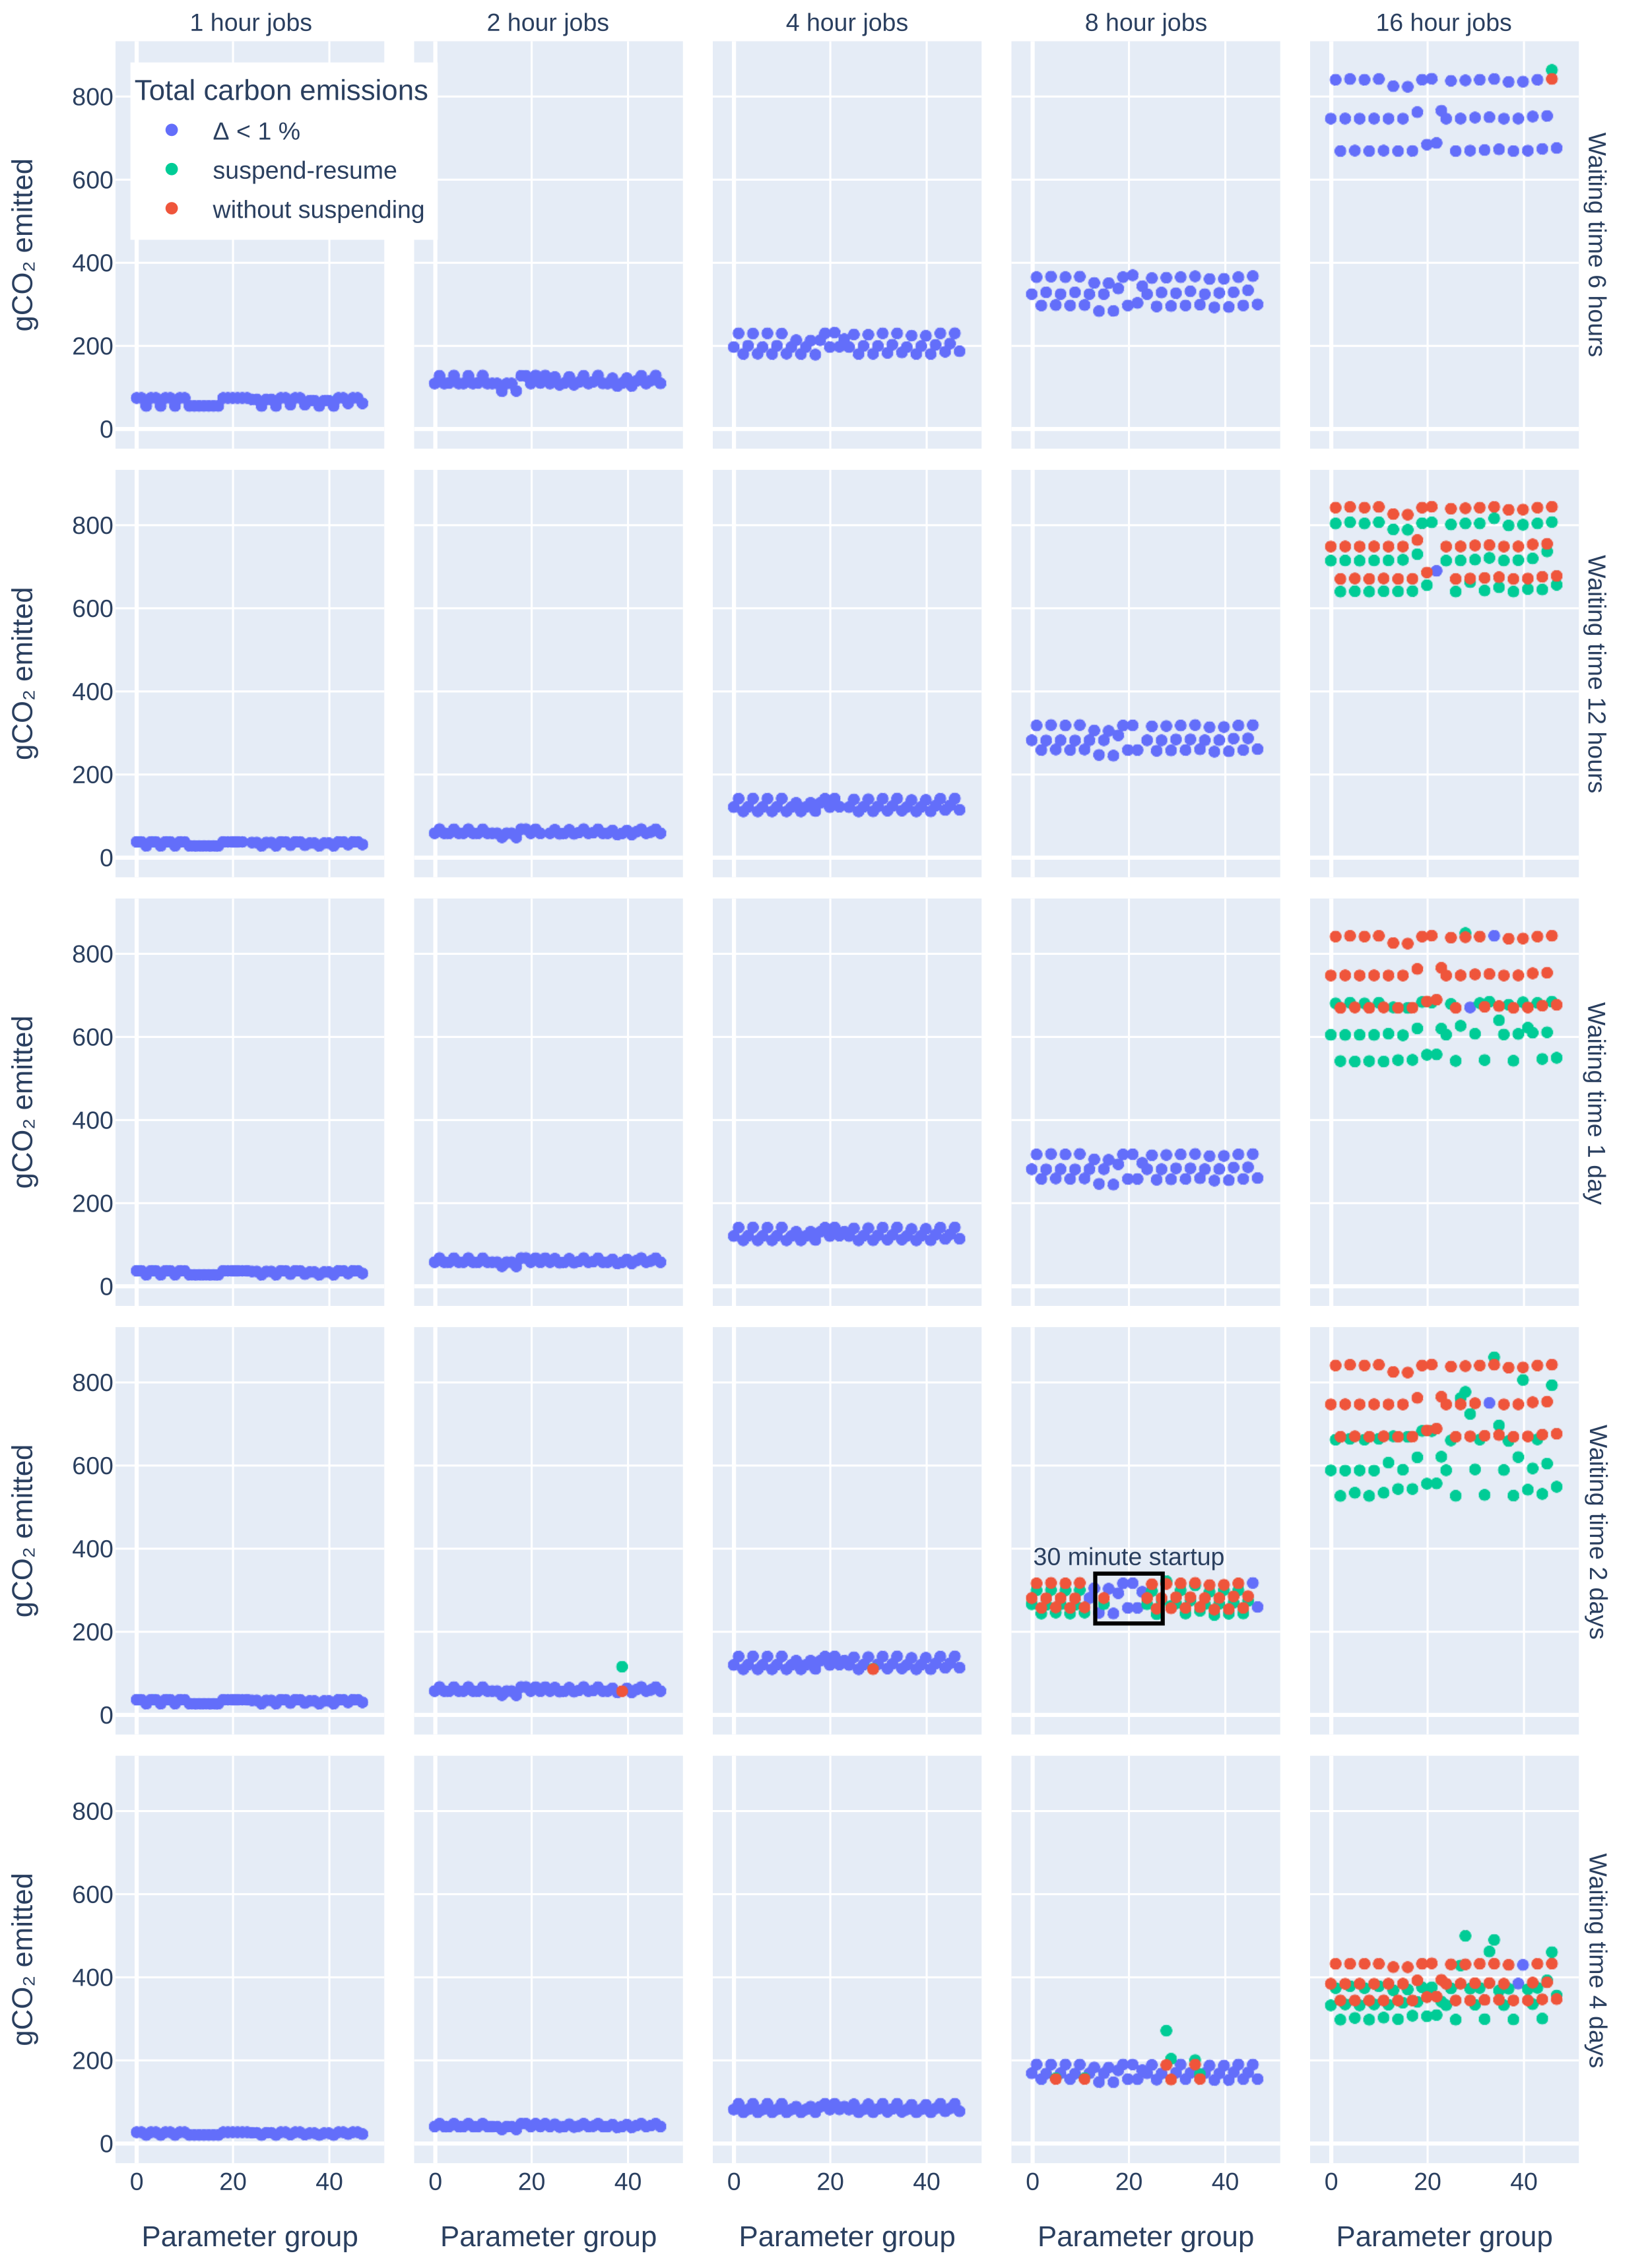
\includegraphics[width=\linewidth]{GAIA/notebooks/eval_same_job_different_schedulers.pdf}
    \caption[short]{All simulated jobs and their total carbon emissions, compared between the two scheduling approaches. Blue indicates equal emissions, red and green differentiate the schedulers. The combination of startup length, startup power and phases is encoded on the x-axis. Savings from adopting a suspend \& resume strategy are only noticeable for very long jobs with long waiting times.}
    \label{fig:eval_different_schedulers}
\end{figure}

\begin{figure}
    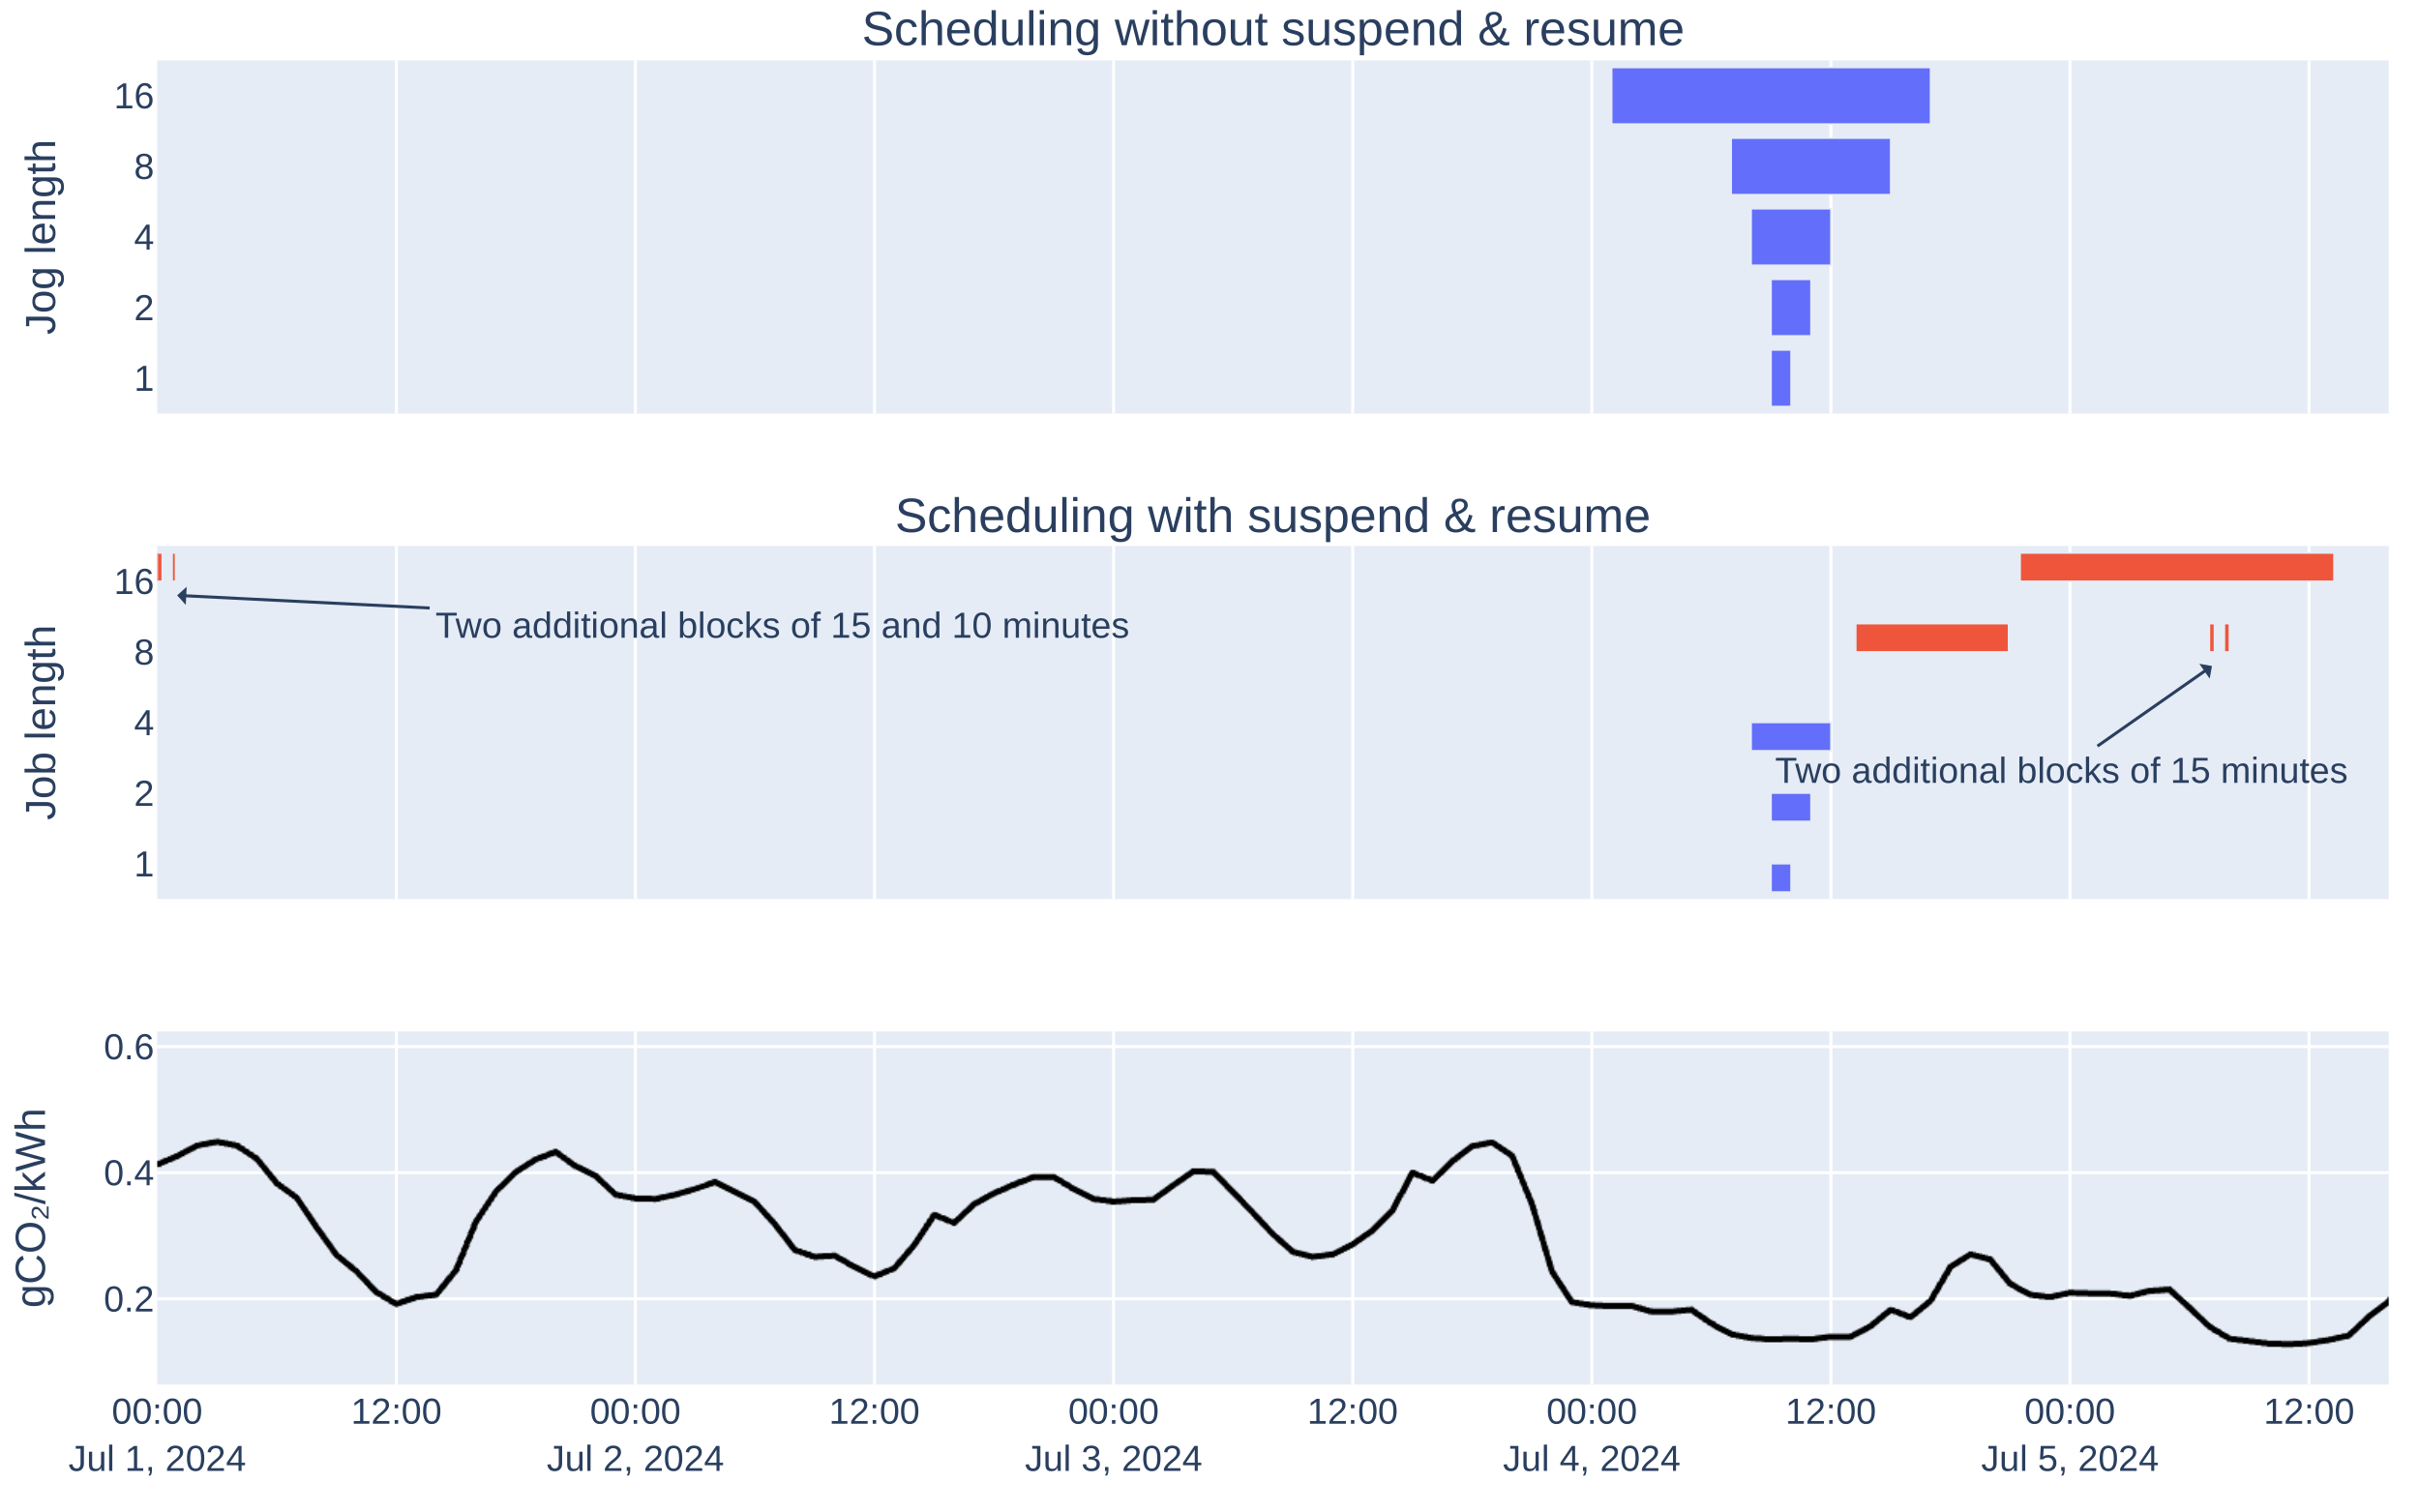
\includegraphics[width=\linewidth]{GAIA/notebooks/timelimited_gantt.pdf}
    \caption[short]{Schedules of jobs with different lengths under different schedulers. All jobs have a waiting time of 4 days and a startup time of 5 minutes and an uneven phase configuration. The red bars are suboptimal schedules that are found upon being time limited.}
    \label{fig:timelimited_gantt}
\end{figure}

\begin{figure}
    \includegraphics[width=\linewidth]{GAIA/slurmlogs/gap_value_ecdf.pdf}
    \caption[short]{Cumulative distribution plot of the 209 gap values of time limited schedules. A higher gap indicates worse results. There is a heavy skew to 100\%, with half of the values being above 95\%}
    \label{fig:ecdf_gap}
\end{figure}

\todo[inline]{Write how the current evaluation is kinda not working too well for the given research question, and how a better experiment could be done.}

\section{Effect of Phases}

\begin{figure}
    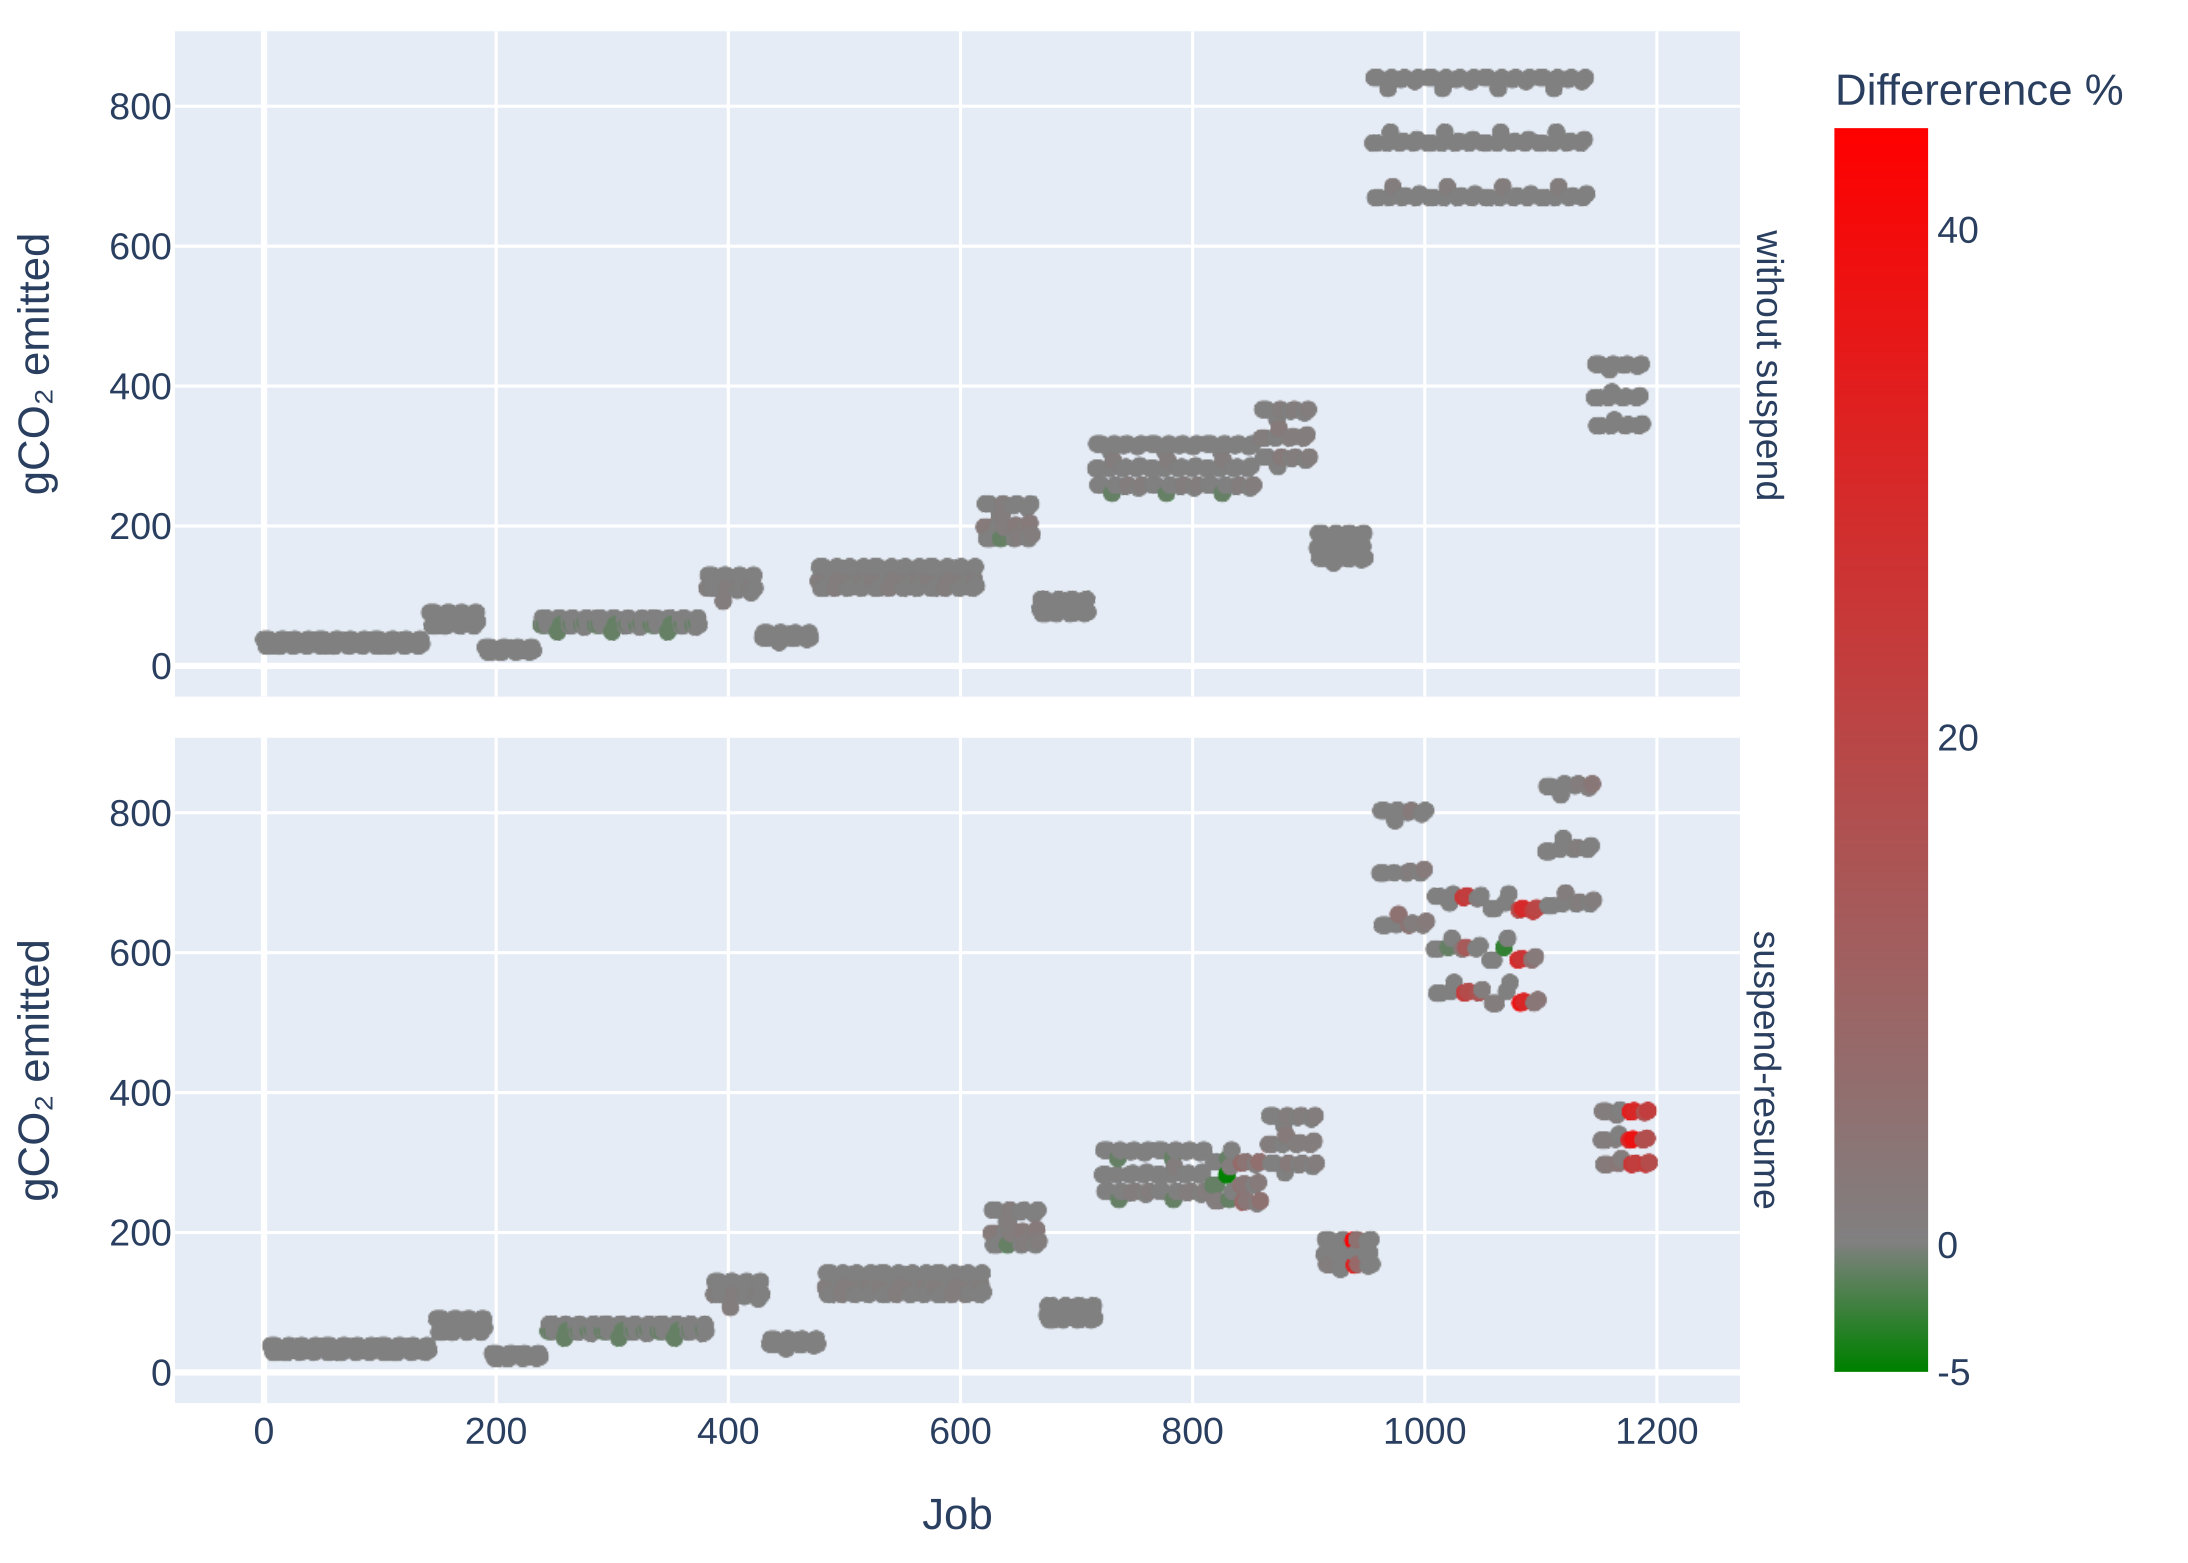
\includegraphics[width=\linewidth]{GAIA/notebooks/eval_same_job_different_phases.pdf}
    \caption[short]{Difference carbon emissions from having heterogeneous phases instead of a constant average. For the majority of jobs, this had an effect of ±1\%. There are also some jobs for the suspend \& resume strategy, where this increased carbon emissions. These are however likely due to time-outs due to increased complexity}

    \label{fig:different_phases_no_effect_lol}
\end{figure}

\section{Effect of Waiting Times}

\begin{figure}
    \includegraphics[width=\linewidth]{GAIA/notebooks/eval_same_job_different_deadlines.pdf}
    \caption[short]{Carbon-costs of Jobs under different waiting times. Each Group shares all remaining parameters.
    With increased waiting times, the carbon costs tend to go down. Each dot represents the lowest time a specific carbon-emission can be hit, so if two waiting times result in the same emissions, only the lower is plotted.}

    \label{fig:eval_different_deadlines}
\end{figure}
